\documentclass[]{beamer}
\usepackage{etex}
\usepackage{beamerthemesplit}
\usepackage{graphics,epsfig}
\usepackage{pstricks}
\usepackage{graphicx}
\usepackage{hyperref}
\usepackage{subfigure}
\usepackage{multirow}
\usepackage{xspace}
\usepackage{listings}
\usepackage{tikz}


\mode<presentation>
{ \usetheme{Boadilla}
  \setbeamercovered{transparent}
  \setbeamertemplate{items}[circle]
  \setbeamertemplate{theorems}[numbered]
  \setbeamertemplate{footline}[frame number]
}
 
%\useinnertheme[shadow=true]{rounded}
\useoutertheme{shadow}
\usecolortheme{whale}

\newcommand\blfootnote[1]{
  \begingroup
  \renewcommand\thefootnote{}\footnote{#1}
  \addtocounter{footnote}{-1}
  \endgroup
}

\mode
<all>

\title{C Programming}
\author{Wan-Lei Zhao}

\makeatletter
\DeclareRobustCommand\onedot{\futurelet\@let@token\@onedot}


\DeclareMathOperator*{\argmax}{argmax}
\makeatother

\begin{document}
\begin{frame}
   \begin{center}
    \vspace{24pt}
    \Huge\textbf{C Programming}\blfootnote{Email: wlzhao@xmu.edu.cn, copyrights are fully reserved by the author.}\\
     \Huge{Lecture 7: struct, union and enum}
     \begin{table}
     \scriptsize{
     	\begin{tabular}{|c|c|c|}\hline
     	Name&Gender&Age \\\hline\hline
     	Tom & \textcolor{blue}{Male} & 22 \\\hline
     	Jack& \textcolor{blue}{Male} &21 \\\hline
     	Jane& \textcolor{blue}{Female} & 21 \\\hline
     	\end{tabular}
     	}
     \end{table}
    \vspace{36pt}
  \end{center}
  \begin{align*}
   \vspace{18pt}
      \large{\mbox{Lecturer:}~Dr.~\mbox{Wan-Lei~~Zhao}} \\
      \large{Spring~~Semester~~2022} \\
   \vspace{30pt}
  \end{align*}
\end{frame}

\definecolor{cornblue}{HTML}{6495ED}
\definecolor{navyblue}{HTML}{000080}
\definecolor{midnblue}{HTML}{191970}
\definecolor{lghtblue}{HTML}{B0C4DE}
\setbeamercolor{background}{fg=black, bg=lghtblue}
\setbeamercolor{palette primary}{fg=white, bg=lghtblue}
\setbeamercolor{palette secondary}{fg=black, bg=cornblue}
\setbeamercolor{palette tertiary}{fg=black, bg=lghtblue}
\setbeamercolor{palette quaternary}{fg=black, bg=lghtblue}
\setbeamercolor{frametitle}{fg=black, bg=white}
\definecolor{ballblue}{rgb}{0.13, 0.67, 0.8}
\definecolor{cornflowerblue}{rgb}{0.39,0.58,0.93}
\definecolor{babyblueeyes}{rgb}{0.63, 0.79, 0.95}

\setbeamertemplate{footline}
{
  \leavevmode%
  \hbox{%
  \begin{beamercolorbox}[wd=.275\paperwidth,ht=2.25ex,dp=1ex,center]{author in head/foot}%
    \usebeamerfont{author in head/foot}\insertshortauthor
  \end{beamercolorbox}%
  \begin{beamercolorbox}[wd=.44\paperwidth,ht=2.25ex,dp=1ex,center]{title in head/foot}%
    \usebeamerfont{title in head/foot}\insertshorttitle\hspace*{3em}
    \hspace*{1ex}
  \end{beamercolorbox}%
  \begin{beamercolorbox}[wd=.285\paperwidth,ht=2.25ex,dp=1ex,center]{date/foot}%
    \usebeamerfont{title in head/foot}\hspace*{2em}
    \insertframenumber{} / \inserttotalframenumber\hspace*{1ex}
  \end{beamercolorbox}}%
  \vskip0pt
}



% preset-listing options
\lstset{
  backgroundcolor=\color{white},   
  basicstyle=\footnotesize,    
  language=c,
  breakatwhitespace=false,         
  breaklines=true,                 % sets automatic line breaking
  captionpos=b,                    % sets the caption-position to bottom
  commentstyle=\color{ballblue},    % comment style
  extendedchars=true,              
  frame=single,                    % adds a frame around the code     
  keywordstyle=\color{blue},       % keyword style
  numbers=left,                    
  numbersep=5pt,                   
  numberstyle=\tiny\color{blue}, 
  rulecolor=\color{babyblueeyes},
  stepnumber=1,              
  stringstyle=\color{black},     % string literal style
  tabsize=4,                       % sets default tabsize to 4 spaces
  title=\lstname                   
}


\begin{frame}[fragile]{Opening Discussion}
\begin{itemize}
	\item {Given we have following informatio for \textit{40} students}
	\begin{enumerate}
		\item {student number}
		\item {name}
		\item {age}
		\item {gender}
		\item {height}
		\item {GPA}
	\end{enumerate}
	\item {We now want to build records for all the students}
\end{itemize}
\begin{lstlisting}[linewidth=0.7\linewidth, xleftmargin=0.05\linewidth]
int main()
{
    char std1nm[64], std2nm[64], ...;
    char std1nb[11], std2nb[11], ...;
    int  std1ag, std2ag, ...;
    char std1gd[5], std1gd[5], ...;
    ...
}
\end{lstlisting}
\end{frame}

\section{struct}
\label{sec:structs}
\begin{frame}<beamer>
    \frametitle{Outline}
    \tableofcontents[currentsection]
\end{frame}

\begin{frame}[fragile]{Composite Data Types}
\begin{itemize}
	\item {It is valid/OK to do it in the way we learned}
	\item {However, it is not convenient}
	\item {C provides us the way to extend current data types}
	\item {We can combine primitive types into one type}
\end{itemize}
\begin{columns}
\begin{column}{0.2\linewidth}
\end{column}
\begin{column}{0.4\linewidth}
\begin{lstlisting}
struct STD {
   char stdNm[64];
   char stdNb[11];
   int  age;
   char gender[5];
};
\end{lstlisting}
\end{column}
\begin{column}{0.2\linewidth}
\end{column}
\end{columns}
\begin{itemize}
	\item {``\textcolor{blue}{struct} STD'' is a new data type}
	\item {Its role is similar as \textcolor{blue}{int}, or \textcolor{blue}{float},...}
\end{itemize}
\end{frame}

\begin{frame}[fragile]{struct: grammar of definition}
\begin{center}
	\Large{
	\textcolor{blue}{struct} \textcolor{red}{structTag} \{ \\
	  \textcolor{blue}{type1} member1; \\
	  \textcolor{blue}{type2} member2; \\
	   ... \\
	  \textcolor{blue}{typeN} memberN; \};
	}
\end{center}
\begin{itemize}
	\item {Keyword ``\textcolor{blue}{struct}'' is required, it tells C you are going to define a composite type}
	\item {\textcolor{red}{structTag} gives a \textbf{unique} tag for this new type}
	\item {You list all the memebers and their corresponding types}
	\item {``\textcolor{red}{;}'' is required at the end}
	\item {Keep in your mind, you define a \textbf{type} instead of a variable/constant}
\end{itemize}
\end{frame}

\begin{frame}[fragile]{struct: define variable of composite type (1)}
\begin{center}
	\Large{
	\textcolor{blue}{struct} \textcolor{red}{structTag} \textbf{record};
	}
\end{center}
\begin{itemize}
	\item {Keyword ``\textcolor{blue}{struct}''  and \textcolor{red}{structTag} are required}
	\item {``record'' is the variable name of \textcolor{red}{structTag} type}
\end{itemize}
\end{frame}

\begin{frame}[fragile]{struct: define variable of composite type (2)}
\begin{center}
	\Large{
	\textcolor{blue}{struct} \textcolor{red}{structTag} \textbf{record};
	}
\end{center}
\begin{itemize}
	\item {Keyword ``\textcolor{blue}{struct}''  and \textcolor{red}{structTag} are required}
	\item {``record'' is the variable name of \textcolor{red}{structTag} type}
\end{itemize}
\begin{lstlisting}
struct STD {
   char stdNm[64];
   char stdNb[11];
   int  age;
   char gender[5];
};
int main()
{
   struct STD record;
   struct STD stds[40];
}
\end{lstlisting}
\end{frame}

\begin{frame}[fragile]{struct: initialize variable of composite type (1)}
\begin{itemize}
	\item {Each memember in the composite type variable is treated as a variable}
	\item {They are visited via ``var.member1''}
\end{itemize}
\begin{lstlisting}[linewidth=0.7\linewidth, xleftmargin=0.05\linewidth]
struct STD {
   char stdNm[64];
   char stdNb[11];
   int  age;
   char gender[5];
};
int main()
{
   struct STD record;
   strcpy(record.stdNm, "Min Li");
   strcpy(record.stdNb, "11201522031");
   record.age = 20;
   strcpy(record.gender, "male");
}
\end{lstlisting}
\end{frame}

\begin{frame}[fragile]{struct: initialize variable of composite type (2)}
\vspace{-0.15in}
\begin{lstlisting}
#include <stdio.h>
#include <string.h>
struct STD {
   char stdNm[64];
   char stdNb[11];
   int  age;
   char gender[5];};
int main()
{
   struct STD std;
   strcpy(std.stdNm, "Min Li");
   strcpy(std.stdNb, "22031");
   std.age = 20;
   strcpy(std.gender, "male");
   printf("Name: %s\n", std.stdNm);
   printf("Numb: %s\n", std.stdNb);
   printf("Age: %d\n", std.age);
   printf("Gender: %s\n", std.gender);
}
\end{lstlisting}
\end{frame}

\begin{frame}[fragile]{struct: exmaple (1)}
\begin{itemize}
	\item {Please build a struct type for date (Year, month and day)}
	\item {Work out which day it is of the year}
	\begin{enumerate}
		\item {We need \textcolor{blue}{struct} type to keep date inform}
		\item {We need to calculate which day of the year is}
		\item {It depends on year (whether it is a leap year)}
		\item {Depends on the month}
		\item {Depends on the date}
	\end{enumerate}
\end{itemize}
\begin{center}
	\Large{
	   5 minutes to think about it...
	}
\end{center}
\end{frame}

\begin{frame}[fragile]{struct: exmaple (2)}

[General procedure]
\begin{enumerate}
	\item {Accept input, save the information to a date structure}
	\item {Check whether the year is leap year or not}
	\item {Check which month it is}
	\item {We need an array to keep the days of months}
\end{enumerate}

\end{frame}

\begin{frame}[fragile]{struct: exmaple (3)}

[General procedure in more detail]
\begin{enumerate}
	\item {Define a date struct}
	\item {Accept input, save the information to a date structure}
	\item {Initialize of days of months (12 months)}
	\item {If it is leap year and date.month $>=$ 3}
	\item {~~Plus 1 day to the total}
	\item {End-If}
	\item {For i from 1 to (date.month-1)}
	\item {~~sum up days of months before current month}
	\item {End-for}
\end{enumerate}

\end{frame}

\begin{frame}[fragile]{struct: exmaple (4)}
\vspace{-0.22in}
\begin{columns}
\begin{column}{0.48\linewidth}
\begin{lstlisting}
struct DATE {
   int day, month, year;
};

int main()
{
   struct DATE date;
   int dyMonth[]={31,28,31,
   30,31,30,31,31,
   30,31,30,31};
   int i = 1, dayth = 0;
   printf("Year:");
   scanf("%d", &date.year);
   printf("Month:");
   scanf("%d", &date.month);
   printf("Day:");
   scanf("%d", &date.day);
\end{lstlisting}
\end{column}
\begin{column}{0.48\linewidth}
\begin{lstlisting}[firstnumber=17]
   if(isLeap(date.year))
   {
      dayth += 1;
   }
   for(;i<date.month;i++)
   {
      dayth+= dyMonth[i-1];
   }
   dayth += date.day;
   return 0;
}
\end{lstlisting}
\end{column}
\end{columns}
\vspace{-0.15in}
\textcolor{red}{Is there anything wrong?? Two mistakes!!}
\end{frame}

\begin{frame}[fragile]{struct: exmaple (5)}
\vspace{-0.15in}
\begin{columns}
\begin{column}{0.48\linewidth}
\begin{lstlisting}
struct DATE {
   int day, month, year;
};
int isLeap(int year)
{  if(year%4==0) {
      if(year%400==0){
         return 1;
      }else if(year%100=0){
         return 0;
      }
      return 1;
   }else{
      return 0;
   }//end-if-else
}//end-isLeap
int main()
{  struct DATE date;
   int dyMonth[]={31,28,31,
   30,31,30,31,31,
   30,31,30,31};
\end{lstlisting}
\end{column}
\begin{column}{0.48\linewidth}
\begin{lstlisting}[firstnumber=21]
   int i = 1, dayth = 0;
   printf("Year:");
   scanf("%d", &date.year);
   printf("Month:");
   scanf("%d", &date.month);
   printf("Day:");
   scanf("%d", &date.day);
   if(isLeap(date.year)&&date.month>2)
   {
      dayth += 1;
   }
   for(;i<date.month;i++)
   {
      dayth+= dyMonth[i-1];
   }
   dayth += date.day;
   return 0;
}
\end{lstlisting}
\end{column}
\end{columns}
\end{frame}


\begin{frame}[fragile]{struct: size of the struct type (1)}
\begin{itemize}
	\item {Now let's consider another problem}
	\item {What is the size (bytes occupied) of struct type variable}
\end{itemize}
\begin{columns}
\begin{column}{0.48\linewidth}
\begin{lstlisting}
struct DATE {
   int day, month, year;
};
struct STD{
   char Name[10];
   int age;
   char gender[6];
};
int main()
{  
   printf("%d\n", sizeof(struct DATE));
   printf("%d\n", sizeof(struct STD));
   return 0;
}
\end{lstlisting}
\end{column}
\begin{column}{0.48\linewidth}
[Output]
\begin{lstlisting}
12
24
\end{lstlisting}
\begin{itemize}
	\item {Can you figure out why?}
\end{itemize}
\end{column}
\end{columns}
\end{frame}

\begin{frame}[fragile]{struct: size of the struct type (2)}
\begin{itemize}
	\item {Now let's consider another problem}
	\item {What is the size (bytes occupied) of struct type variable}
\end{itemize}
\begin{columns}
\begin{column}{0.48\linewidth}
\begin{lstlisting}
struct DATE {
   int day, month, year;
};
struct STD{
   char Name[10];
   int age;
   char gender[6];
};
int main()
{  
   printf("%d\n", sizeof(struct DATE));
   printf("%d\n", sizeof(struct STD));
   return 0;
}
\end{lstlisting}
\end{column}
\begin{column}{0.48\linewidth}
[Output]
\begin{lstlisting}
12
24
\end{lstlisting}
\begin{itemize}
	\item {\textcolor{green}{Name} will be given with \textcolor{red}{12} bytes instead of 10}
	\item {\textcolor{green}{gender} will be given with \textcolor{red}{8} bytes instead of 6}
	\item {For the convevience of memory allocation}
	\item {This could be different from one compiler to another}
\end{itemize}
\end{column}
\end{columns}
\end{frame}


\begin{frame}[fragile]{struct: \textcolor{blue}{typedef} to save code (1)}
\begin{itemize}
	\item {In ``struct STD'',  ``\textcolor{blue}{struct}'' has been repeated everywhere}
	\item {We can use ``\textcolor{blue}{typedef}'' to save up our typing}
\end{itemize}
\vspace{-0.15in}
\begin{columns}
\begin{column}{0.48\linewidth}
\begin{lstlisting}
struct DATE {
   int day, month, year;
};
struct STD{
   char Name[10];
   int age;
   char gender[6];
};
typedef struct STD StdType;
typedef struct DATE DatType;
int main()
{  
   DatType date;
   StdType std;
   printf("%d\n", sizeof(DatType));
   ...
}
\end{lstlisting}
\end{column}
\begin{column}{0.48\linewidth}
\begin{itemize}
	\item {During compiling stage}
	\item {``StdType'' is replaced by ``\textcolor{blue}{struct} STD''}
\end{itemize}
\end{column}
\end{columns}
\end{frame}

\begin{frame}[fragile]{struct: \textcolor{blue}{typedef} to save code (2)}
\begin{itemize}
	\item {You can apply \textcolor{blue}{typedef} to any type}
\end{itemize}
\vspace{-0.05in}
\begin{lstlisting}
#include <stdio.h>
typedef unsigned int uint;

int main()
{
   uint a = 32768;
   printf("%d\n", a);
   printf("%d\n", sizeof(uint));
   return 0;
}
\end{lstlisting}
\begin{itemize}
	\item {During compiling stage}
	\item {``uint'' is replaced by ``\textcolor{blue}{unsigned int}''}
	\item {You actually give a \textbf{nickname} to the type by \textcolor{blue}{typedef}}
\end{itemize}
\end{frame}



\section{union}
\label{sec:union}
\begin{frame}<beamer>
    \frametitle{Outline}
    \tableofcontents[currentsection]
\end{frame}

\begin{frame}[fragile]{union}
\begin{itemize}
	\item {Sometimes it is not necessary to reserve a field for each struct member}
	\item {Several fields are allowed to share the same block of memory}
	\item {This special type of structure is called \textcolor{blue}{union}}
\end{itemize}
\begin{columns}
\begin{column}{0.45\linewidth}
\begin{lstlisting}
struct Data {
   short i;
   float f;
   char str[20];
};
\end{lstlisting}
\end{column}
\begin{column}{0.45\linewidth}
\begin{lstlisting}
union Data {
   short i;
   float f;
   char str[20];
};
\end{lstlisting}
\end{column}
\end{columns}
\end{frame}

\begin{frame}[fragile]{union: definition (1)}
\begin{center}
	\Large{
   \textcolor{blue}{union} [union tag] \{ \\
   \textcolor{blue}{type1} member1; \\
   \textcolor{blue}{type2} member2; \\
   ... \\
   \};
	}
\end{center}
\begin{itemize}
	\item {It is basically very similar as \textcolor{blue}{struct}}
	\item {However, the members are kept in different way}
\end{itemize}
\begin{columns}
\begin{column}{0.45\linewidth}
\begin{lstlisting}
struct Data1 {
   short i;
   float f;
   char str[20];
};
\end{lstlisting}
\end{column}
\begin{column}{0.45\linewidth}
\begin{lstlisting}
union Data2 {
   short i;
   float f;
   char str[20];
};
\end{lstlisting}
\end{column}
\end{columns}
\end{frame}

\begin{frame}[fragile]{union: definition (2)}
\vspace{-0.2in}
\begin{lstlisting}
struct Data1 {
   short i;
   float f;
   char str[10];
};

union Data2 {
   short i;
   float f;
   char str[10];
};
int main()
{
   Data1 d1;
   Data2 d2;
   printf("Size of d1 %d", sizeof(d1));
   printf("Size of d2 %d", sizeof(d2));
   return 0;
}
\end{lstlisting}
\vspace{-0.15in}
[Output:???]
\end{frame}

\begin{frame}[fragile]{union: definition (3)}
\begin{lstlisting}
int main()
{
   Data1 d1;
   Data2 d2;
   printf("Size of d1 %d", sizeof(d1));
   printf("Size of d2 %d", sizeof(d2));
   return 0;
}
\end{lstlisting}
\begin{center}
Size of d1: 20 \\
Size of d2: 12
\end{center}
\begin{itemize}
	\item {Can you figure out why??}
\end{itemize}
\end{frame}

\begin{frame}[fragile]{union: definition (4)}
\begin{lstlisting}
int main()
{
   Data1 d1;
   Data2 d2;
   printf("Size of d1 %d", sizeof(d1));
   printf("Size of d2 %d", sizeof(d2));
   return 0;
}
\end{lstlisting}
\begin{center}
Size of d1: 20 \\
Size of d2: 12
\end{center}
\begin{itemize}
	\item {For the convenience of memory allocation}
	\item {\textcolor{green}{str} will be given \textcolor{red}{12} bytes instead of 10}
\end{itemize}
\end{frame}

\begin{frame}[fragile]{union: how they are kept in the memory}
\begin{figure}
	\subfigure[struct]
	{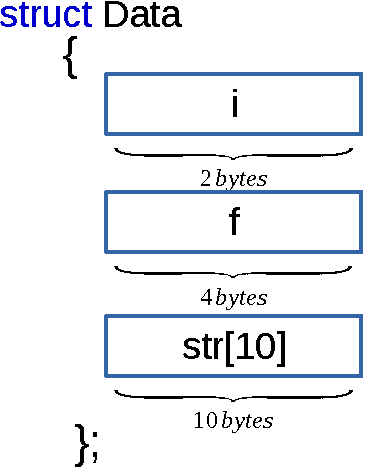
\includegraphics[width=0.25\linewidth]{figs/struct.pdf}}
	\hspace{0.15in}
	\subfigure[union]
	{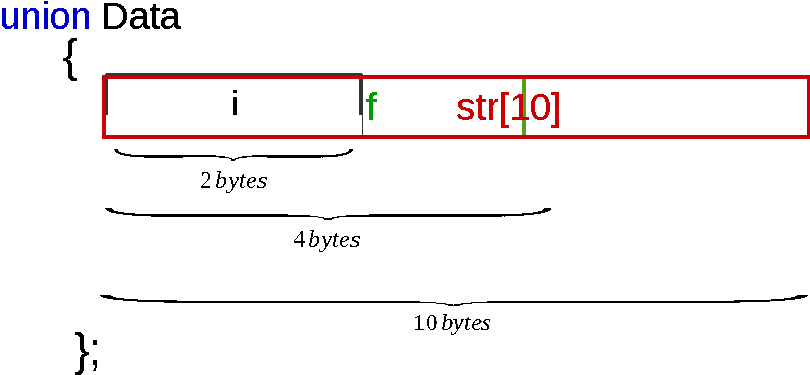
\includegraphics[width=0.6\linewidth]{figs/union.pdf}}
\end{figure}
\end{frame}

\begin{frame}[fragile]{union: learn by example (1)}
\begin{lstlisting}
#include <stdio.h>
#include <string.h>
union Data {
   int i;
   float f;
   char str[20];
};
int main() 
{
   union Data data;        
   data.i = 10;
   data.f = 220.5;
   strcpy( data.str, "C Programming");

   printf( "data.i : %d\n", data.i);
   printf( "data.f : %f\n", data.f);
   printf( "data.str : %s\n", data.str);
   return 0;
}
\end{lstlisting}
\begin{itemize}
	\item {See what the output??}
\end{itemize}
\end{frame}

\begin{frame}[fragile]{union: learn by example (2)}
\vspace{-0.2in}
\begin{lstlisting}
#include <stdio.h>
#include <string.h>
union Data {
   int i;
   float f;
   char str[20];
};
int main(){
   union Data data;        
   data.i = 10;
   data.f = 220.5;
   strcpy( data.str, "C Programming");
   printf( "data.i : %d\n", data.i);
   printf( "data.f : %f\n", data.f);
   printf( "data.str : %s\n", data.str);
}
\end{lstlisting}
\vspace{-0.20in}
data.i : 1917853763\\
data.f : 4122360580327794860452759994368.000000\\
data.str : C Programming
\end{frame}

\begin{frame}[fragile]{union: learn by example (3)}
\vspace{-0.2in}
\begin{lstlisting}
#include <stdio.h>
#include <string.h>
union Data {
   int i;
   float f;
   char str[20];
};
int main(){
   union Data data;        
   data.i = 10;
   strcpy( data.str, "C Programming");
   data.f = 220.5;
   printf( "data.i : %d\n", data.i);
   printf( "data.f : %f\n", data.f);
   printf( "data.str : %s\n", data.str);
}
\end{lstlisting}

\end{frame}

\begin{frame}[fragile]{union: learn by example (4)}
\vspace{-0.16in}
\begin{lstlisting}
#include <stdio.h>
#include <string.h>
union Data {
   int i;
   float f;
   char str[20];
};
int main(){
   union Data data;        
   data.i = 10;
   strcpy( data.str, "C Programming");
   data.f = 220.5;
   printf( "data.i : %d\n", data.i);
   printf( "data.f : %f\n", data.f);
   printf( "data.str : %s\n", data.str);
}
\end{lstlisting}
\vspace{-0.16in}
data.i : 1130135552 \\
data.f : 220.500000 \\
data.str : 
\end{frame}

\begin{frame}[fragile]{union: learn by example (5)}
\vspace{-0.16in}
\begin{lstlisting}
#include <stdio.h>
#include <string.h>
union Data {
   int i;
   float f;
   char str[20];
};
int main(){
   data.i = 10;
   printf( "data.i : %d\n", data.i);
   data.f = 220.5;
   printf( "data.f : %f\n", data.f);
   strcpy( data.str, "C Programming");
   printf( "data.str : %s\n", data.str);
}
\end{lstlisting}

\end{frame}

\begin{frame}[fragile]{union: learn by example (6)}
\vspace{-0.16in}
\begin{lstlisting}
#include <stdio.h>
#include <string.h>
union Data {
   int i;
   float f;
   char str[20];
};
int main(){
   data.i = 10;
   printf( "data.i : %d\n", data.i);
   data.f = 220.5;
   printf( "data.f : %f\n", data.f);
   strcpy( data.str, "C Programming");
   printf( "data.str : %s\n", data.str);
}
\end{lstlisting}
\vspace{-0.16in}
data.i : 10 \\
data.f : 220.500000 \\
data.str : C Programming
\end{frame}



\section{enum}
\label{sec:enum}
\begin{frame}<beamer>
    \frametitle{Outline}
    \tableofcontents[currentsection]
\end{frame}

\begin{frame}{enum: motivation}
\begin{itemize}
	\item {Sometimes, we feel it is more meaningful }
	\item {with symbols: Janurary, Feburary ,..., December}
	\item {than numbers: 1, 2, ..., 12}
\end{itemize}

\begin{itemize}
	\item {enum allows us to do a kind of correlating}
	\item {Numbers are assigned with readable symbols}
\end{itemize}

\end{frame}

\begin{frame}{enum: definition (1)}
\begin{center}
	\Large{
	   \textcolor{blue}{enum} \textcolor{red}{enumName}\{memb1, memb2, memb3,...\};
	}
\end{center}

\begin{itemize}
	\item {You enumerate all the members' name inside ``\{\}''}
	\item {They are symbols}
	\item {They will be related to integer 0, 1, 2,... automatically}
\end{itemize}

\end{frame}

\begin{frame}[fragile]{enum: definition (2)}
\begin{center}
	\Large{
	   \textcolor{blue}{enum} \textcolor{red}{enumName}\{memb1, memb2, memb3\};
	}
\end{center}
\begin{lstlisting}
enum Month {Jan, Feb, Mar, Apr, May, Jun, Jul, Aug, Sep, Oct, Nov, Dec};
int main()
{
   ...
}
\end{lstlisting}
\begin{itemize}
	\item {You enumerate all the members' name inside ``\{\}''}
	\item {They are symbols}
	\item {They will be related to integer 0, 1, 2,... automatically}
\end{itemize}
\end{frame}


\begin{frame}[fragile]{enum: how to use it}
\begin{lstlisting}
#include <stdio.h>
enum Month {Jan, Feb, Mar, Apr, May, Jun, Jul, Aug, Sep, Oct, Nov, Dec};
int main()
{
   enum Month m;
   m = Feb;
   printf("Month is: %d\n", m);
   return 0;
}
\end{lstlisting}
[Output]
\begin{lstlisting}
Month is: 1
\end{lstlisting}
\begin{itemize}
	\item {\textbf{Feb} is a symbol instead of a string}
	\item {They will be related to integer 0, 1, 2,... automatically}
\end{itemize}

\end{frame}

\begin{frame}[fragile]{enum: learn by example (1)}
\begin{columns}
\begin{column}{0.52\linewidth}
\begin{lstlisting}
#include <stdio.h>
enum Week {Mon=1, Tue=1, Wed=3,
 Thu=5, Fri, Sat=4, Sun};
int main()
{
   enum Week wk;
   wk=Wed;
   printf("Wed: %d\n", wk);
   wk=Fri;
   printf("Fri: %d\n", wk);
   wk=Sun;
   printf("Sun: %d\n", wk);
   return 0;
}
\end{lstlisting}
\end{column}
\begin{column}{0.43\linewidth}
[Output]
\begin{lstlisting}
Wed: ?
Fri: ?
Sun: ?
\end{lstlisting}
\end{column}
\end{columns}
\end{frame}

\begin{frame}[fragile]{enum: learn by example (2)}
\begin{columns}
\begin{column}{0.52\linewidth}
\begin{lstlisting}
#include <stdio.h>
enum Week {Mon=1, Tue=1, Wed=3,
 Thu=5, Fri, Sat=4, Sun};
int main()
{
   enum Week wk;
   wk=Wed;
   printf("Wed: %d\n", wk);
   wk=Fri;
   printf("Fri: %d\n", wk);
   wk=Sun;
   printf("Sun: %d\n", wk);
   return 0;
}
\end{lstlisting}
\end{column}
\begin{column}{0.43\linewidth}
[Output]
\begin{lstlisting}
Wed: 3
Fri: 6
Sun: 5
\end{lstlisting}
\end{column}
\end{columns}
\begin{itemize}
	\item {Can you figure out why??}
	\item {This way is valid, but NOT \textcolor{red}{suggested}}
\end{itemize}
\end{frame}

\begin{frame}[fragile]{enum: learn by example (2)}
\begin{columns}
\begin{column}{0.52\linewidth}
\begin{lstlisting}
#include <stdio.h>
enum Week {Mon=1, Tue, Wed,
 Thu, Fri, Sat, Sun};
int main()
{
   enum Week wk;
   wk=Wed;
   printf("Wed: %d\n", wk);
   wk=Fri;
   printf("Fri: %d\n", wk);
   wk=Sun;
   printf("Sun: %d\n", wk);
   return 0;
}
\end{lstlisting}
\end{column}
\begin{column}{0.43\linewidth}
[Output]
\begin{lstlisting}
Wed: 3
Fri: 5
Sun: 7
\end{lstlisting}
\end{column}
\end{columns}
\begin{itemize}
	\item {This is the right way}
\end{itemize}
\end{frame}

\begin{frame}[fragile]{enum: learn by example (3)}
\begin{columns}
\begin{column}{0.52\linewidth}
\begin{lstlisting}
#include <stdio.h>
enum Week {Mon=1, Tue, Wed,
 Thu, Fri, Sat, Sun};
typedef enum Week WkType;
int main()
{
   WkType wk;
   wk=Wed;
   printf("Wed: %d\n", wk);
   wk=Fri;
   printf("Fri: %d\n", wk);
   wk=Sun;
   printf("Sun: %d\n", wk);
   return 0;
}
\end{lstlisting}
\end{column}
\begin{column}{0.43\linewidth}
[Output]
\begin{lstlisting}
Wed: 3
Fri: 5
Sun: 7
\end{lstlisting}
\end{column}
\end{columns}
\begin{itemize}
	\item {You can use ``\textcolor{blue}{typedef}'' to save up your coding efforts}
\end{itemize}
\end{frame}

\section{}
\end{document}
